\documentclass[symmetric, justified, a4paper]{tufte-book}

%% configuration, packages

% Switch this variable true/false to print or hide lecturer notes.
\newcommand{\printlecnotes}{true}

\usepackage{colortbl} 

\hypersetup{colorlinks}% uncomment this line if you prefer colored hyperlinks (e.g., for onscreen viewing)

%% TODO add logic for quasar / orange name change

\usepackage{import}

%%
% If they're installed, use Bergamo and Chantilly from www.fontsite.com.
% They're clones of Bembo and Gill Sans, respectively.
%\IfFileExists{bergamo.sty}{\usepackage[osf]{bergamo}}{}% Bembo
%\IfFileExists{chantill.sty}{\usepackage{chantill}}{}% Gill Sans

%\usepackage{microtype}

\usepackage{tcolorbox}
\usepackage[english]{babel}

%%
% For nicely typeset tabular material
\usepackage{booktabs}

% For stacking images
\usepackage{stackengine}

\usepackage{wrapfig}
\setlength{\wrapoverhang}{5.5cm} % this is something we can set in future to whatever the exact position is

%%
% For graphics / images
\usepackage{graphicx}
%\setkeys{Gin}{width=\linewidth,totalheight=\textheight,keepaspectratio}  % disabled for problems with scale/resolution
\setkeys{Gin}{keepaspectratio}

\graphicspath{{graphics/}}

% The fancyvrb package lets us customize the formatting of verbatim
% environments.  We use a slightly smaller font.
\usepackage{fancyvrb}
\usepackage{hyperref}
\fvset{fontsize=\normalsize}

%%
% Sets the name of the package between Orange compilations
% Always use this instead of directly referring to Orange or Quasar or Oasys, etc.
\newcommand{\mutation}{Orange}
% \newcommand{\mutation}{scOrange}
% \newcommand{\mutation}{Quasar}
\newcommand{\widget}[1]{\textsl{#1}}
\newcommand{\wn}{~cm$^{-1}$}

%%
% Prints argument within hanging parentheses (i.e., parentheses that take
% up no horizontal space).  Useful in tabular environments.
\newcommand{\hangp}[1]{\makebox[0pt][r]{(}#1\makebox[0pt][l]{)}}

%%
% Prints an asterisk that takes up no horizontal space.
% Useful in tabular environments.
\newcommand{\hangstar}{\makebox[0pt][l]{*}}

%%
% Prints a trailing space in a smart way.
\usepackage{xspace}

\newcommand{\TL}{Tufte-\LaTeX\xspace}

% Prints the month name (e.g., January) and the year (e.g., 2008)
\newcommand{\monthyear}{%
  \ifcase\month\or January\or February\or March\or April\or May\or June\or
  July\or August\or September\or October\or November\or
  December\fi\space\number\year
}


% Prints an epigraph and speaker in sans serif, all-caps type.
\newcommand{\openepigraph}[2]{%
  %\sffamily\fontsize{14}{16}\selectfont
  \begin{fullwidth}
  \sffamily\large
  \begin{doublespace}
  \noindent\allcaps{#1}\\% epigraph
  \noindent\allcaps{#2}% author
  \end{doublespace}
  \end{fullwidth}
}

% Inserts a blank page
\newcommand{\blankpage}{\newpage\hbox{}\thispagestyle{empty}\newpage}

\usepackage{units}

% Typesets the font size, leading, and measure in the form of 10/12x26 pc.
\newcommand{\measure}[3]{#1/#2$\times$\unit[#3]{pc}}

% Macros for typesetting the documentation
\newcommand{\hlred}[1]{\textcolor{Maroon}{#1}}% prints in red
\newcommand{\hangleft}[1]{\makebox[0pt][r]{#1}}
\newcommand{\hairsp}{\hspace{1pt}}% hair space
\newcommand{\hquad}{\hskip0.5em\relax}% half quad space
\newcommand{\TODO}{\textcolor{red}{\bf TODO!}\xspace}
\newcommand{\ie}{\textit{i.\hairsp{}e.}\xspace}
\newcommand{\eg}{\textit{e.\hairsp{}g.}\xspace}
\newcommand{\na}{\quad--}% used in tables for N/A cells
\providecommand{\XeLaTeX}{X\lower.5ex\hbox{\kern-0.15em\reflectbox{E}}\kern-0.1em\LaTeX}
\newcommand{\tXeLaTeX}{\XeLaTeX\index{XeLaTeX@\protect\XeLaTeX}}
% \index{\texttt{\textbackslash xyz}@\hangleft{\texttt{\textbackslash}}\texttt{xyz}}
\newcommand{\tuftebs}{\symbol{'134}}% a backslash in tt type in OT1/T1
\newcommand{\doccmdnoindex}[2][]{\texttt{\tuftebs#2}}% command name -- adds backslash automatically (and doesn't add cmd to the index)
\newcommand{\doccmddef}[2][]{%
  \hlred{\texttt{\tuftebs#2}}\label{cmd:#2}%
  \ifthenelse{\isempty{#1}}%
    {% add the command to the index
      \index{#2 command@\protect\hangleft{\texttt{\tuftebs}}\texttt{#2}}% command name
    }%
    {% add the command and package to the index
      \index{#2 command@\protect\hangleft{\texttt{\tuftebs}}\texttt{#2} (\texttt{#1} package)}% command name
      \index{#1 package@\texttt{#1} package}\index{packages!#1@\texttt{#1}}% package name
    }%
}% command name -- adds backslash automatically
\newcommand{\doccmd}[2][]{%
  \texttt{\tuftebs#2}%
  \ifthenelse{\isempty{#1}}%
    {% add the command to the index
      \index{#2 command@\protect\hangleft{\texttt{\tuftebs}}\texttt{#2}}% command name
    }%
    {% add the command and package to the index
      \index{#2 command@\protect\hangleft{\texttt{\tuftebs}}\texttt{#2} (\texttt{#1} package)}% command name
      \index{#1 package@\texttt{#1} package}\index{packages!#1@\texttt{#1}}% package name
    }%
}% command name -- adds backslash automatically
\newcommand{\docopt}[1]{\ensuremath{\langle}\textrm{\textit{#1}}\ensuremath{\rangle}}% optional command argument
\newcommand{\docarg}[1]{\textrm{\textit{#1}}}% (required) command argument
\newenvironment{docspec}{\begin{quotation}\ttfamily\parskip0pt\parindent0pt\ignorespaces}{\end{quotation}}% command specification environment
\newcommand{\docenv}[1]{\texttt{#1}\index{#1 environment@\texttt{#1} environment}\index{environments!#1@\texttt{#1}}}% environment name
\newcommand{\docenvdef}[1]{\hlred{\texttt{#1}}\label{env:#1}\index{#1 environment@\texttt{#1} environment}\index{environments!#1@\texttt{#1}}}% environment name
\newcommand{\docpkg}[1]{\texttt{#1}\index{#1 package@\texttt{#1} package}\index{packages!#1@\texttt{#1}}}% package name
\newcommand{\doccls}[1]{\texttt{#1}}% document class name
\newcommand{\docclsopt}[1]{\texttt{#1}\index{#1 class option@\texttt{#1} class option}\index{class options!#1@\texttt{#1}}}% document class option name
\newcommand{\docclsoptdef}[1]{\hlred{\texttt{#1}}\label{clsopt:#1}\index{#1 class option@\texttt{#1} class option}\index{class options!#1@\texttt{#1}}}% document class option name defined
\newcommand{\docmsg}[2]{\bigskip\begin{fullwidth}\noindent\ttfamily#1\end{fullwidth}\medskip\par\noindent#2}
\newcommand{\docfilehook}[2]{\texttt{#1}\index{file hooks!#2}\index{#1@\texttt{#1}}}
\newcommand{\doccounter}[1]{\texttt{#1}\index{#1 counter@\texttt{#1} counter}}


% do not put empty space before chapters; not needed in this handbook
\titlespacing*{\chapter}{0pt}{0pt}{40pt}

% Allows adding images that go into or over page margins
\newcommand{\infinitewidthbox}[1]{\noindent\makebox[\textwidth]{#1}}

% Generates the index
\usepackage{makeidx}

% Remove "Figure X:" before figures.
% We do not need these in our short chapters.
\usepackage{etoolbox}
\makeatletter
\patchcmd{\@caption}
  {\noindent\csname fnum@#1\endcsname: \ignorespaces}
  {\noindent}
  {}{}
\makeatother

% Do not put additional empty pages before chapters
\makeatletter
\patchcmd{\chapter}{\if@openright\cleardoublepage\else\clearpage\fi}{\clearpage}{}{}
\makeatother


% Lecturer notes
\newtcolorbox{mylecnote}[1][]{%
  size=title,
  boxrule=0.5pt,
  fonttitle={\large\bfseries},
  coltitle={black},
  title={Lecturer note.\ },
  attach title to upper,
  #1
}

\newcommand{\lecnotes}[1]{
	\ifthenelse{\equal{\printlecnotes}{true}}{
	\begin{mylecnote}
		{#1}
	\end{mylecnote}
	}{}
}

%\printnotes{}

\makeindex

%%
% Book metadata
\title{Using \mutation\thanks{Thanks to everyone who worked on this document.}}
\author[Biolab and Collaborators]{Biolab and Collaborators}
\publisher{Biolab}

\begin{document}

% Front matter
\frontmatter

% full title page
\maketitle

% v.4 copyright page
% \iffalse
\newpage
\begin{fullwidth}
~\vfill
\thispagestyle{empty}
\setlength{\parindent}{0pt}
\setlength{\parskip}{\baselineskip}
Copyright \copyright\ \the\year\ \thanklessauthor

\par\smallcaps{Published by \thanklesspublisher}

\par\smallcaps{tufte-latex.googlecode.com}

\par Licensed under the Apache License, Version 2.0 (the ``License''); you may not
use this file except in compliance with the License. You may obtain a copy
of the License at \url{http://www.apache.org/licenses/LICENSE-2.0}. Unless
required by applicable law or agreed to in writing, software distributed
under the License is distributed on an \smallcaps{``AS IS'' BASIS, WITHOUT
WARRANTIES OR CONDITIONS OF ANY KIND}, either express or implied. See the
License for the specific language governing permissions and limitations
under the License.\index{license}

\par\textit{First printing, \monthyear}
\end{fullwidth}

% \fi

\tableofcontents

%\chapter*{Introduction}


\begin{figure*}[t!]
  \includegraphics[width=\linewidth]{graphics/\mutation-intro-fig.jpg}%
  \label{chfig:intro}%
\end{figure*}


\newthought{This book} showcases machine learning and scientific data analysis problems using \mutation\cite{\mutation} through easily reproducible workflows.

First, let us acknowledge that \mutation\ is but a pre-packaged version of Orange\cite{orange} and the Orange Spectroscopy add-on\cite{git\mutation}.

The examples presented here introduce the features of \mutation\ through common data analysis tasks. You will see how common data mining can be accomplished through visual programming. We will also apply the same techniques to spectral data and hyperspectral images. \marginnote{\newthought{These notes include} \mutation\ workflows and visualizations we will construct during the course. 

The original notes were written by the members of the SMIS beam line of the SOLEIL Synchrotron, and the Bioinformatics Lab at University of Ljubljana and are extensions of the notes by Blaž Zupan, Janez Demšar and Marko Toplak.
}
If you are already familiar with data analysis, the methodological aspects of this course will seem simple, but you will have more time to absorb \mutation\ and the \mutation\ philosophy — try to think of what is happening behind the scenes.


\begin{figure*}[b!]
    % \centering
    
\includegraphics[width=30mm]{CC-BY-SA_icon_white.png}
    \label{fig:CC-BY-SA_icon}
\end{figure*}


% Start the main matter (normal chapters)
\mainmatter

%% I would like to have an option of not showing the figure number
%% ? How do we avoid overlapping figure captions?

%%%% ORANGE %%%%

\subimport{chapters/001-workflows/}{workflows}
\subimport{chapters/002-basic-data-exploration/}{basic-data-exploration}
\subimport{chapters/003-saving-your-work/}{saving}
\subimport{chapters/004-loading-data/}{loading-data}

\subimport{chapters/spec-001-spectral-data/}{spectral-data}
\subimport{chapters/spec-010-spectral-pca/}{spectral-pca}
\subimport{chapters/spec-003-hyper-basic/}{hyper-basic}
\subimport{chapters/spec-011-preprocessing/}{spectral-preprocessing}
\subimport{chapters/spec-012-integrals-ratios/}{integrals-ratios}

\subimport{chapters/020-classification/}{classification}
\subimport{chapters/021-classification-trees/}{classification-trees}
\subimport{chapters/022-naive-bayes/}{naive-bayes}
\subimport{chapters/029-classification-accuracy/}{classification-accuracy}

\subimport{chapters/030-how-to-cheat/}{how-to-cheat}
\subimport{chapters/025-random-forests/}{random-forests}
\subimport{chapters/032-cross-validation/}{cross-validation}

% Lesson 18: Hierarchical Clustering
\chapter{Hierarchical Clustering}
\label{ch:hierarchical_clustering}

Say that we are interested in finding clusters in our data. That is, we would like to identify groups of data instances that are close together, similar to each other. Consider a simple, two-featured data set (see the side note) and plot it in the Scatter Plot. How many clusters do we have? What defines a cluster? Which data instances should belong to the same cluster? How does the clustering algorithm actually work?

\begin{marginfigure}
    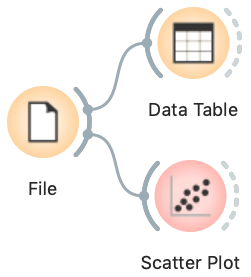
\includegraphics[scale=0.4]{graphics/ch-hierarchical_clustering/workflow_scatterplot.png}
    \caption{We will introduce clustering with a simple data set on students and their grades in English and Algebra.
Load the data set from \url{http://file.biolab.si/text/grades.tab}.}
\end{marginfigure}

First, we need to define what we mean by ``similar''. We will assume that all our data instances are described (profiled) with continuous features. One simple measure of similarity is the Euclidean distance. So, we would like to group data instances with small Euclidean distances.

\begin{figure*}[h]
    \vspace{1cm}
    \centering
    \infinitewidthbox{
    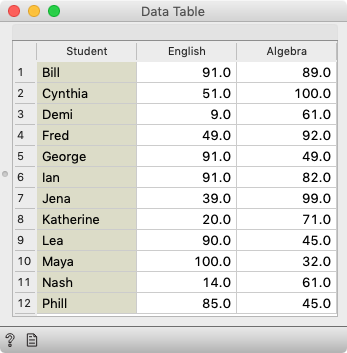
\includegraphics[scale=0.4]{graphics/ch-hierarchical_clustering/grades_table.png}
    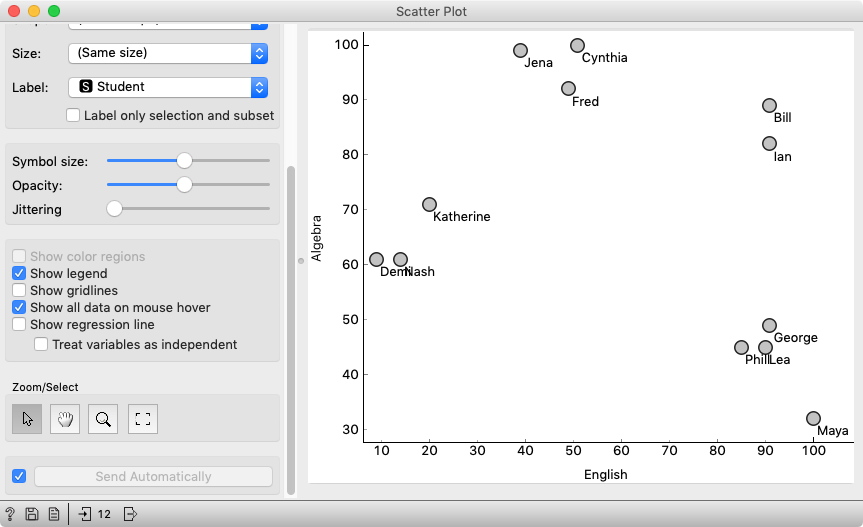
\includegraphics[scale=0.4]{graphics/ch-hierarchical_clustering/grades_scatterplot.png}
    }
    \caption{There are different ways to measure the similarity between clusters. The estimate we have described is called average linkage. We could also estimate the distance through the two closest points in each clusters (single linkage), or through the two points that are furthest away (complete linkage).}
\end{figure*}

Next, we need to define a clustering algorithm. Say that we start with each data instance being its own cluster, and then, at each step, we join the clusters that are closest together. We estimate the distance between the clusters with, say, the average distance between all their pairs of data points. This algorithm is called hierarchical clustering.

\clearpage

One possible way to observe the results of clustering on our small data set with grades is through the following workflow:

\begin{marginfigure}
    \centering
    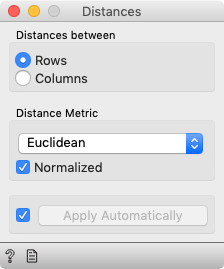
\includegraphics[scale=0.4]{graphics/ch-hierarchical_clustering/distances.png}
\end{marginfigure}

\begin{figure}[h]
    \centering
    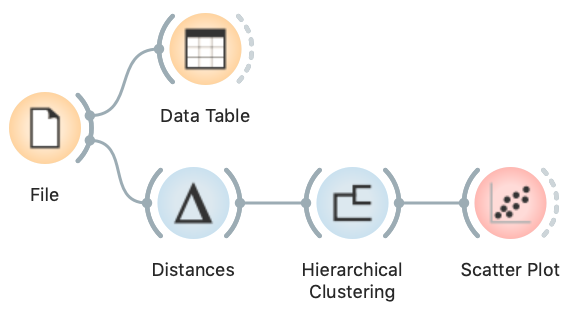
\includegraphics[scale=0.4]{graphics/ch-hierarchical_clustering/workflow_clustering.png}
    \caption{$\;$} % empty caption for proper pagesetting
\end{figure}

Couldn’t be simpler. Load the data, measure the distances, use them in hierarchical clustering, and visualize the results in a scatter plot. The \widget{Hierarchical Clustering} widget allows us to cut the hierarchy at a certain distance score and output the corresponding clusters:

\begin{figure*}[h]
    \centering
    \newcommand{\clustering}{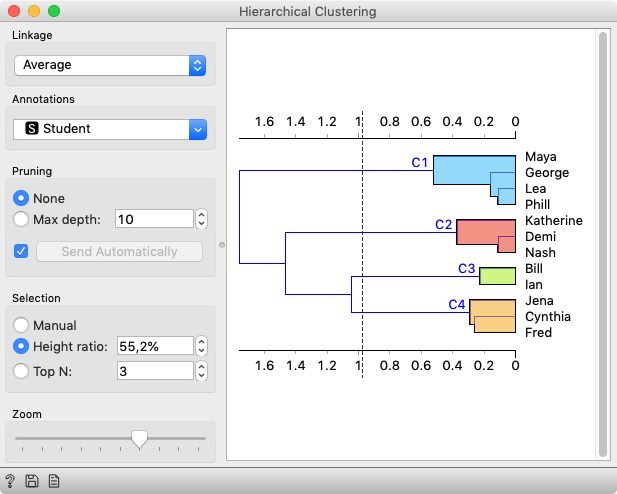
\includegraphics[scale=0.4]{graphics/ch-hierarchical_clustering/hierarchical_clustering.png}}
    \newcommand{\plot}{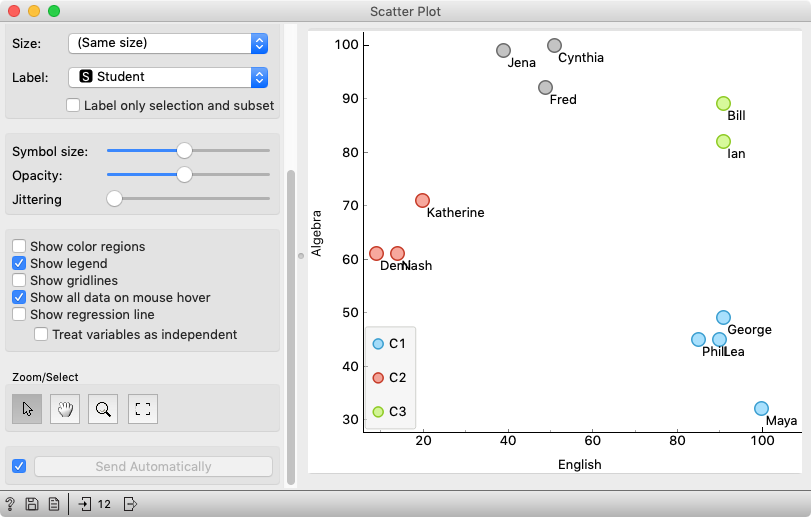
\includegraphics[scale=0.4]{graphics/ch-hierarchical_clustering/scatterplot_clustered.png}}
    \infinitewidthbox{
    \stackinset{r}{-0.5\linewidth}{t}{+0.3\linewidth}{\plot}{\clustering}\hspace{8cm}
    }
\end{figure*}

% Lesson 19: Animal Kingdom
\chapter{Animal Kingdom}
\label{ch:animal_kingdom}

\begin{marginfigure}
    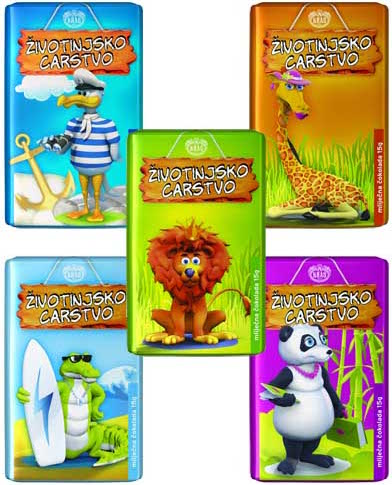
\includegraphics[width=5cm]{graphics/ch-animal_kingdom/kras_zivotinjsko_carstvo.jpg}
\end{marginfigure}

Your lecturers spent a substantial part of their youth admiring a particular Croatian chocolate called Animal Kingdom. Each chocolate bar came with a card---a drawing of some (random) animal, and the associated album made us eat a lot of chocolate.

Funny stuff was we never understood the order in which the cards were laid out in the album. We later learned about taxonomy, but being more inclined to engineering we never mastered learning it in our biology classes. Luckily, there’s data mining and the idea that taxonomy simply stems from measuring the distance between species.

\begin{wrapfigure}{o}{0.8\textwidth}
    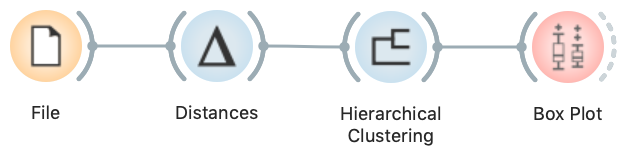
\includegraphics[scale=0.4]{graphics/ch-animal_kingdom/workflow.png}
    \caption{Hierarchical clustering works fast for smaller data sets. But for bigger ones it fails. Simply, it cannot be used. Why?}
\end{wrapfigure}

Here we use zoo data (from the documentation data sets) with attributes that report on various features of animals (has hair, has feathers, lays eggs). We measure the distance and compute the clustering. Animals in this data set are annotated with type (mammal, insect, bird, and so on). It would be cool to know if the clustering re-discovered these groups of animals.

To split the data into clusters, let us manually set a threshold by dragging the vertical line left or right in the visualization. Can you say what is the appropriate number of groups?

\begin{figure*}[h]
    \centering
    \newcommand{\clustering}{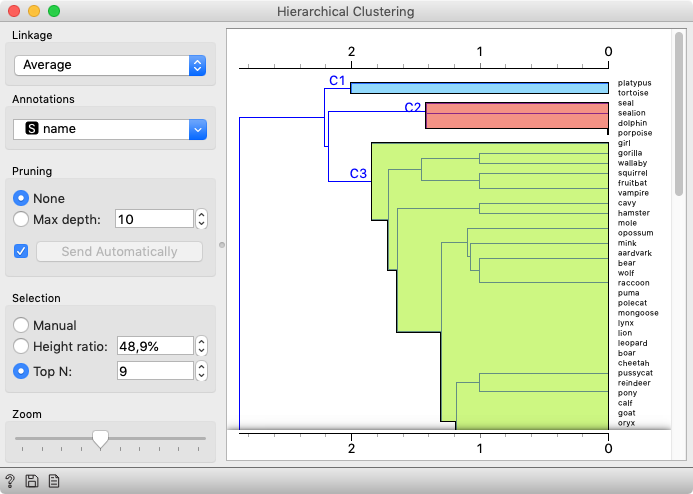
\includegraphics[scale=0.35]{graphics/ch-animal_kingdom/clustering.png}}
    \newcommand{\plot}{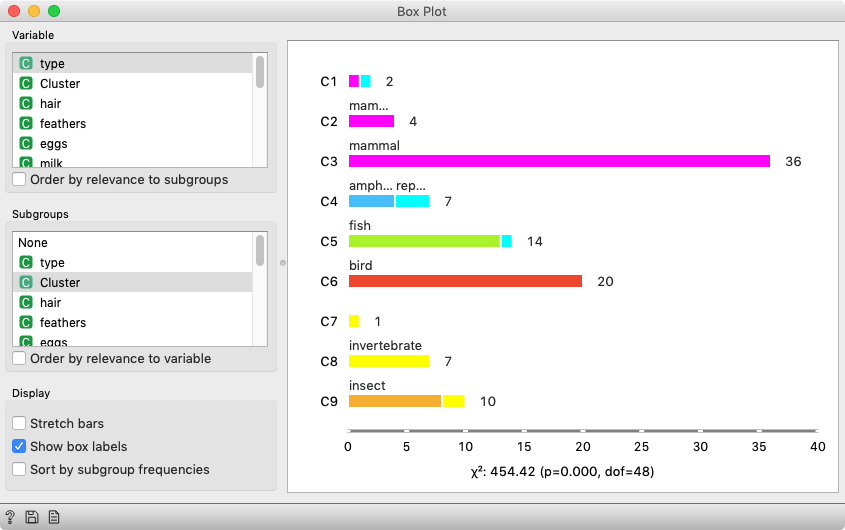
\includegraphics[scale=0.35]{graphics/ch-animal_kingdom/boxplot.png}}
    \infinitewidthbox{
    \stackinset{r}{-0.5\linewidth}{t}{+0.1\linewidth}{\plot}{\clustering}\hspace{8cm}
    }
    \caption{What is wrong with those mammals? Why can't they be in one single cluster? Two reasons. First, they represent 40\% of the data instances. Second, they include some weirdos. Who are they?}
\end{figure*}


% Lesson 20: Classification of Spectra
\chapter{Classification of Spectra}
\label{ch:spectra_classification}

\begin{wrapfigure}{o}{0.82\textwidth}
    \centering
    \vspace{-3.4cm}
    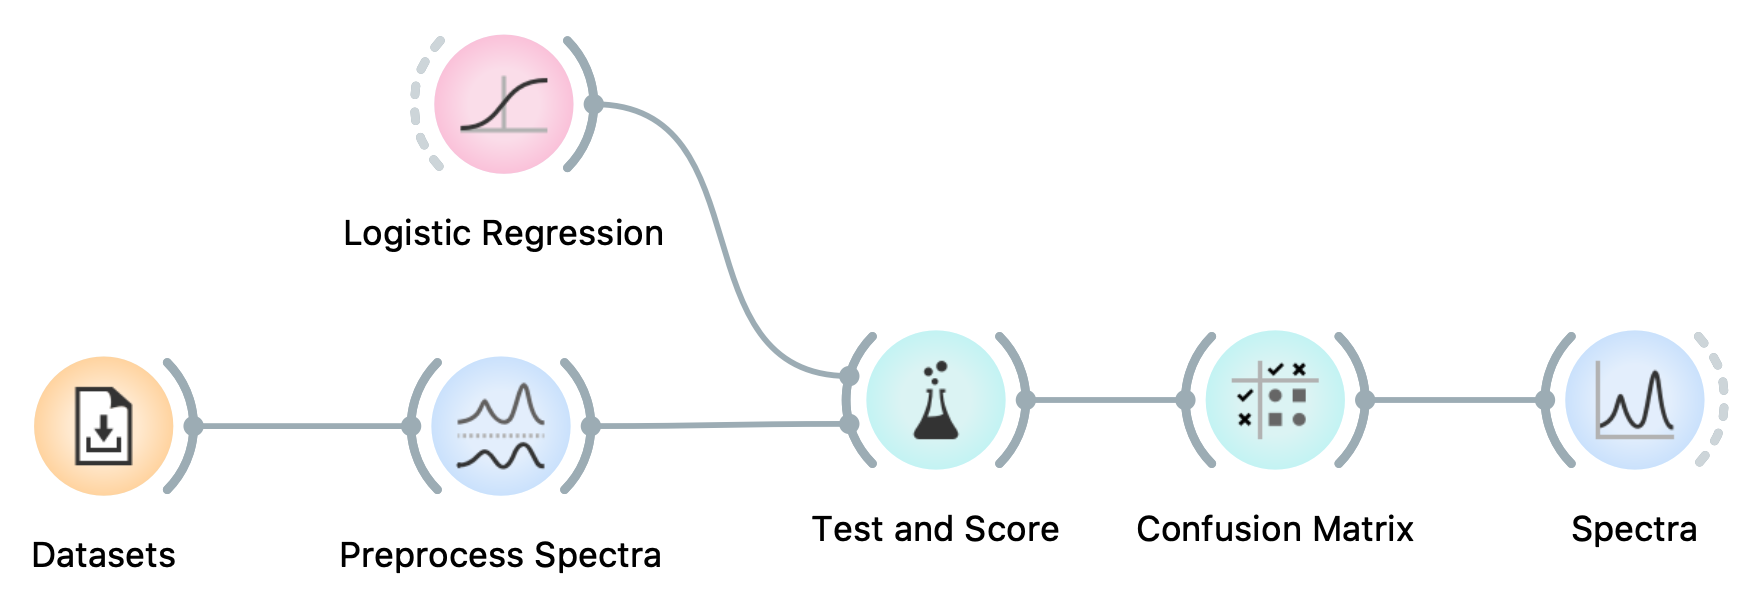
\includegraphics[width=0.95\textwidth]{graphics/ch-spectra_classification/sp_classification-fig1.png}
    \label{fig:spectra_classification-fig1}
\end{wrapfigure}


Let’s open the collagen data set again and see how well can logistic regression predict its four classes. Straightforward, right? Connect \widget{Datasets}, \widget{Logistic Regression}, \widget{Predictions}, \widget{Confusion Matrix} and that's it. We would also like to do some spectral processing (we will only keep the columns for wavenumbers between 1500\wn and 1800\wn).

\begin{figure}[h]
\hspace{-1cm}\stackinset{r}{-0.7\linewidth}{t}{+0.25\linewidth}
  {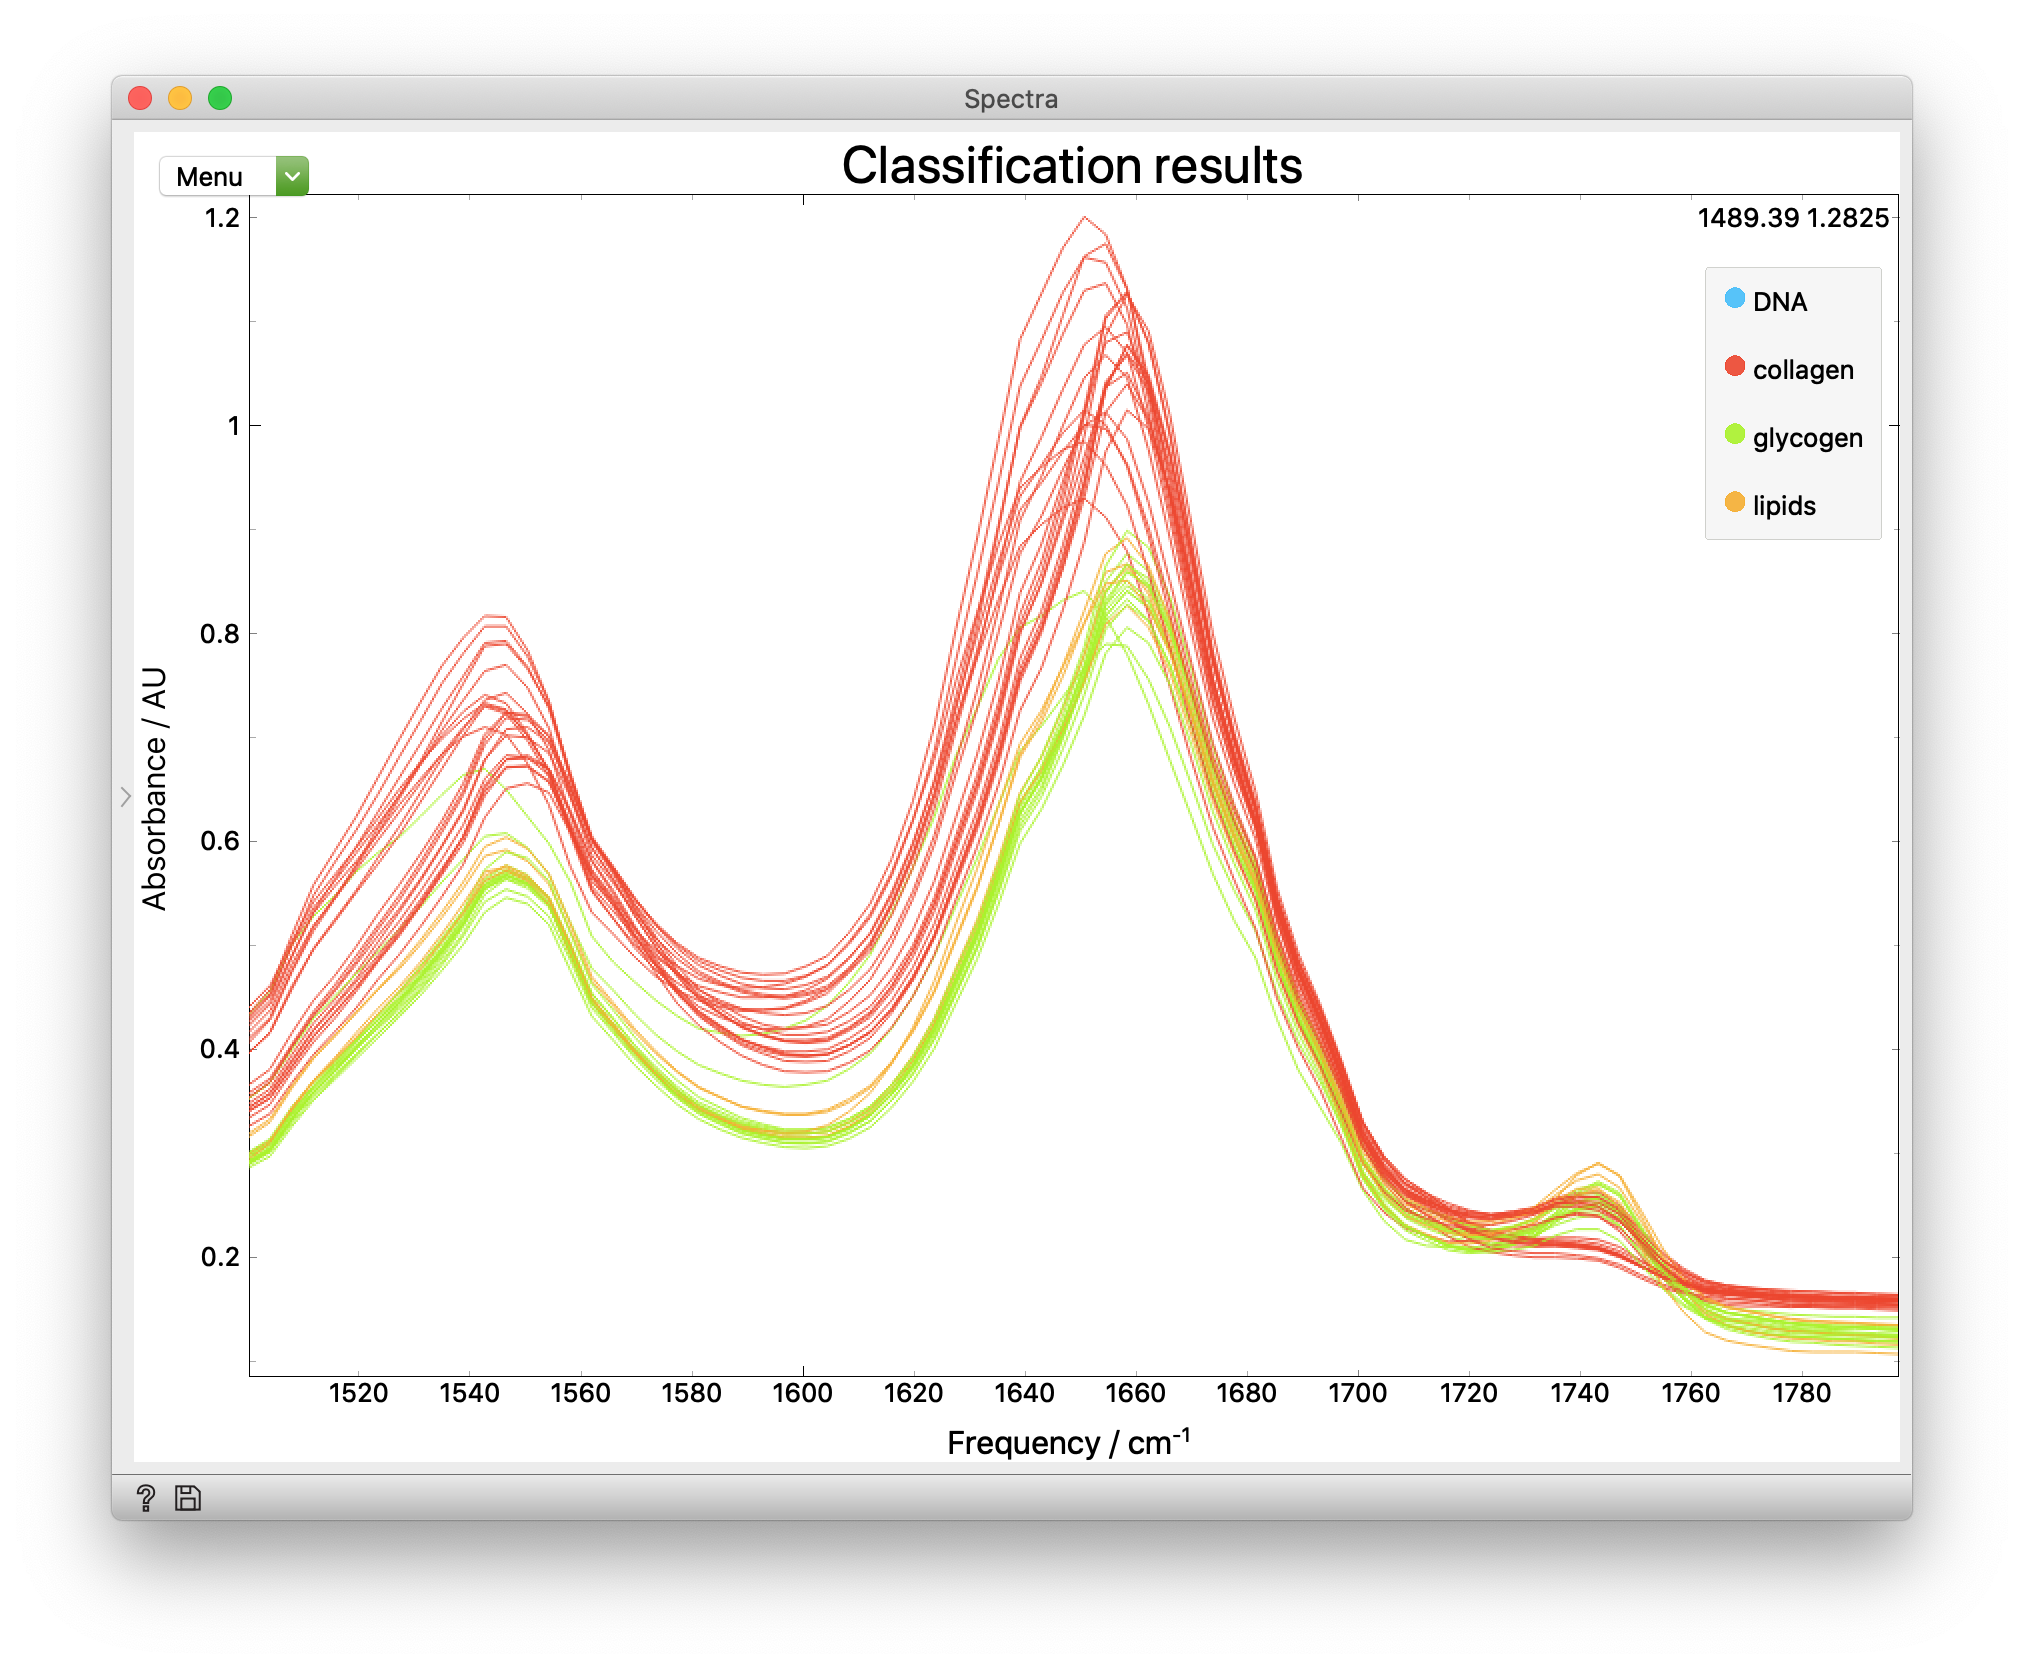
\includegraphics[scale=0.35]{graphics/ch-spectra_classification/sp_classification-fig2b.png}}
  {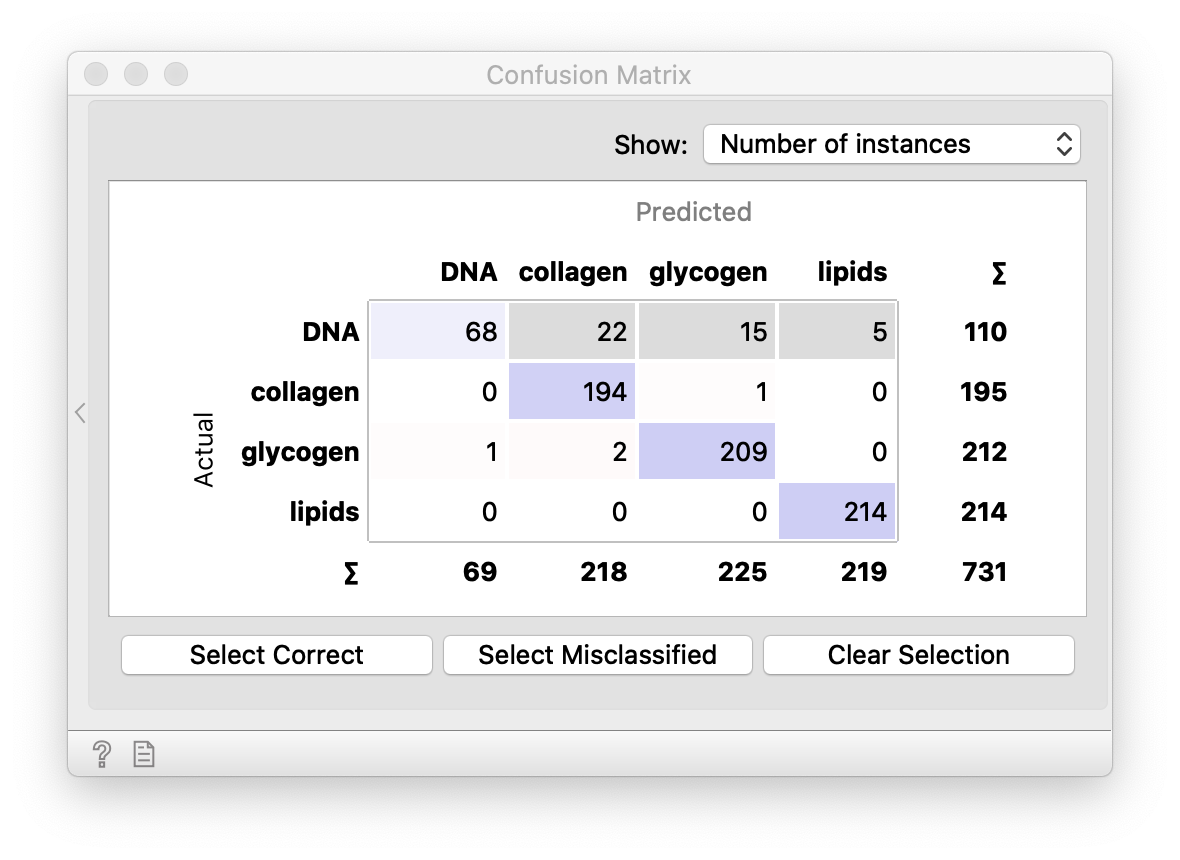
\includegraphics[scale=0.45]{graphics/ch-spectra_classification/sp_classification-fig2a_.png}}
  \caption{The \widget{Spectra} widget shows wrong predictions for the DNA class.}
  \label{fig:spectra_classification-fig2}
\end{figure}

Let’s not forget that it is pointless to predict for the same data as we used for learning. We could either  use a \widget{Data Sampler} and connect its Sample output to \widget{Preprocess Spectra} and Remaining output to \widget{Predictions}, or obtain predictions from the \widget{Test and Score} widget.
\widget{Confusion Matrix} now shows the mistakes of the model (scored with cross-validation). We can select them and inspect them further in a \widget{Spectra} widget. Here we colored them by the predicted class (see the Menu). 

\begin{wrapfigure}{o}{1.1\textwidth}
  \centering
  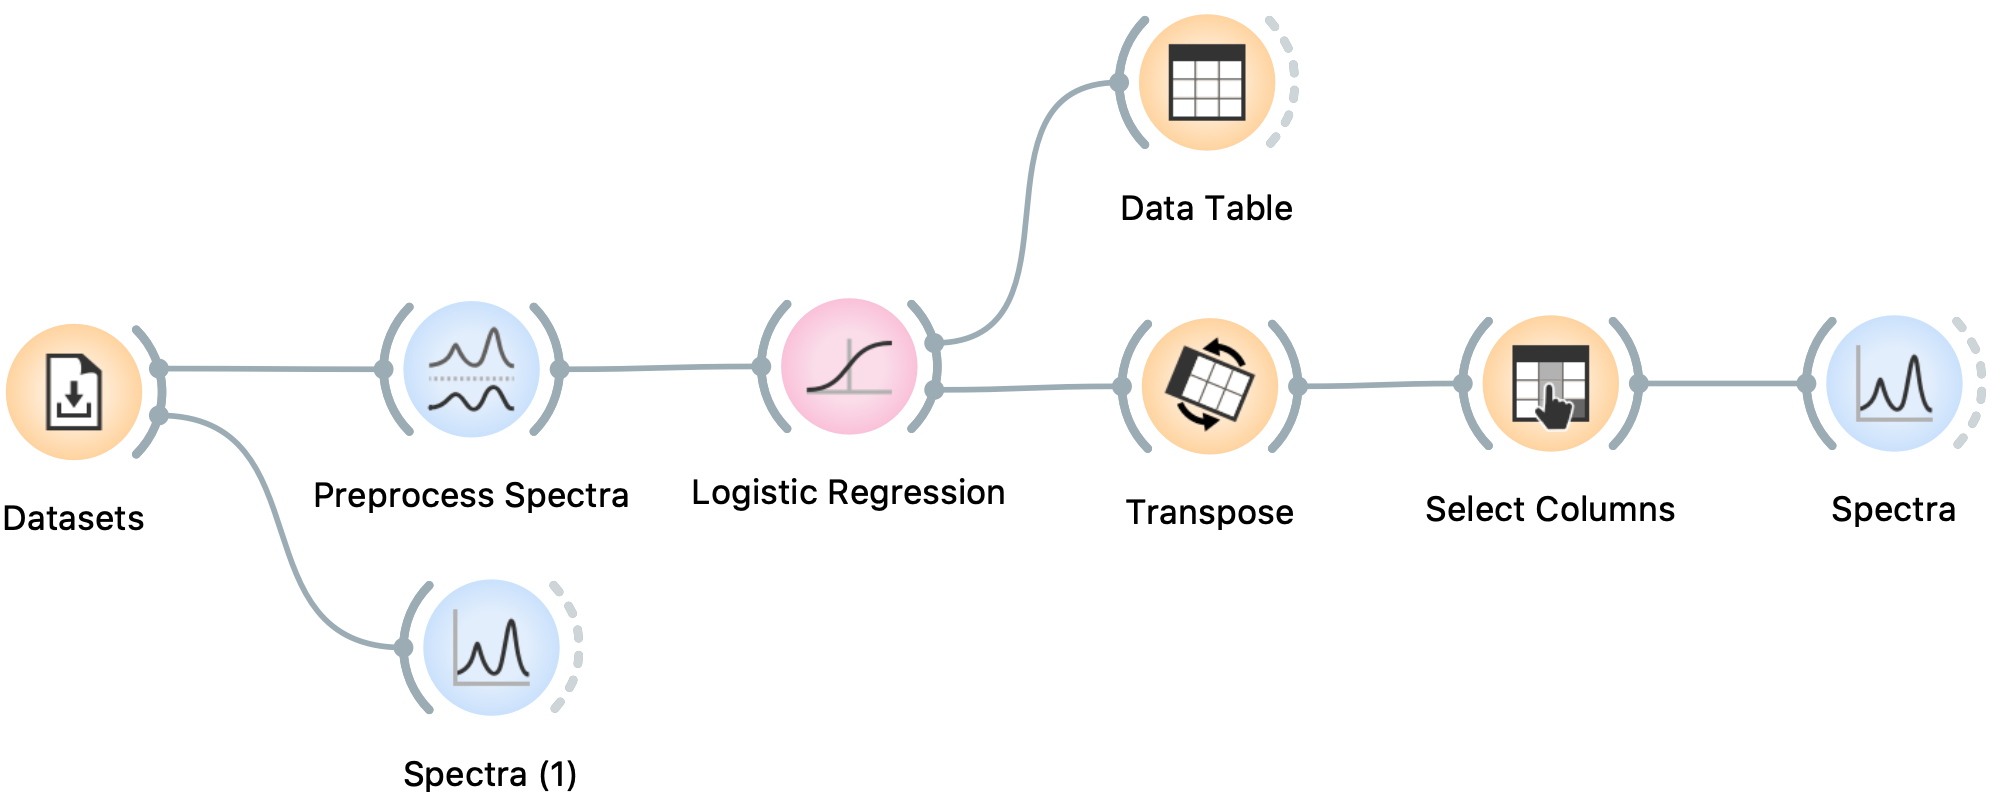
\includegraphics[width=1.1\textwidth]{graphics/ch-spectra_classification/sp_classification-fig3.png}%
  \label{fig:spectra_classification-fig3}
\end{wrapfigure}
But how does the model make its decisions? We already inspected a different model, classification tree, where each node represents a decision on a value of a column.  \widget{Logistic regression} works differently. On the training data it computes weights for all columns (wavelengths), which are then used for prediction, where values are multiplied with weights. To see the weights, connect \widget{Logistic Regression} to a \widget{Data Table}. 

\begin{wrapfigure}{o}{0.9\textwidth}
%  \centering
  \vspace{-0.7cm}
  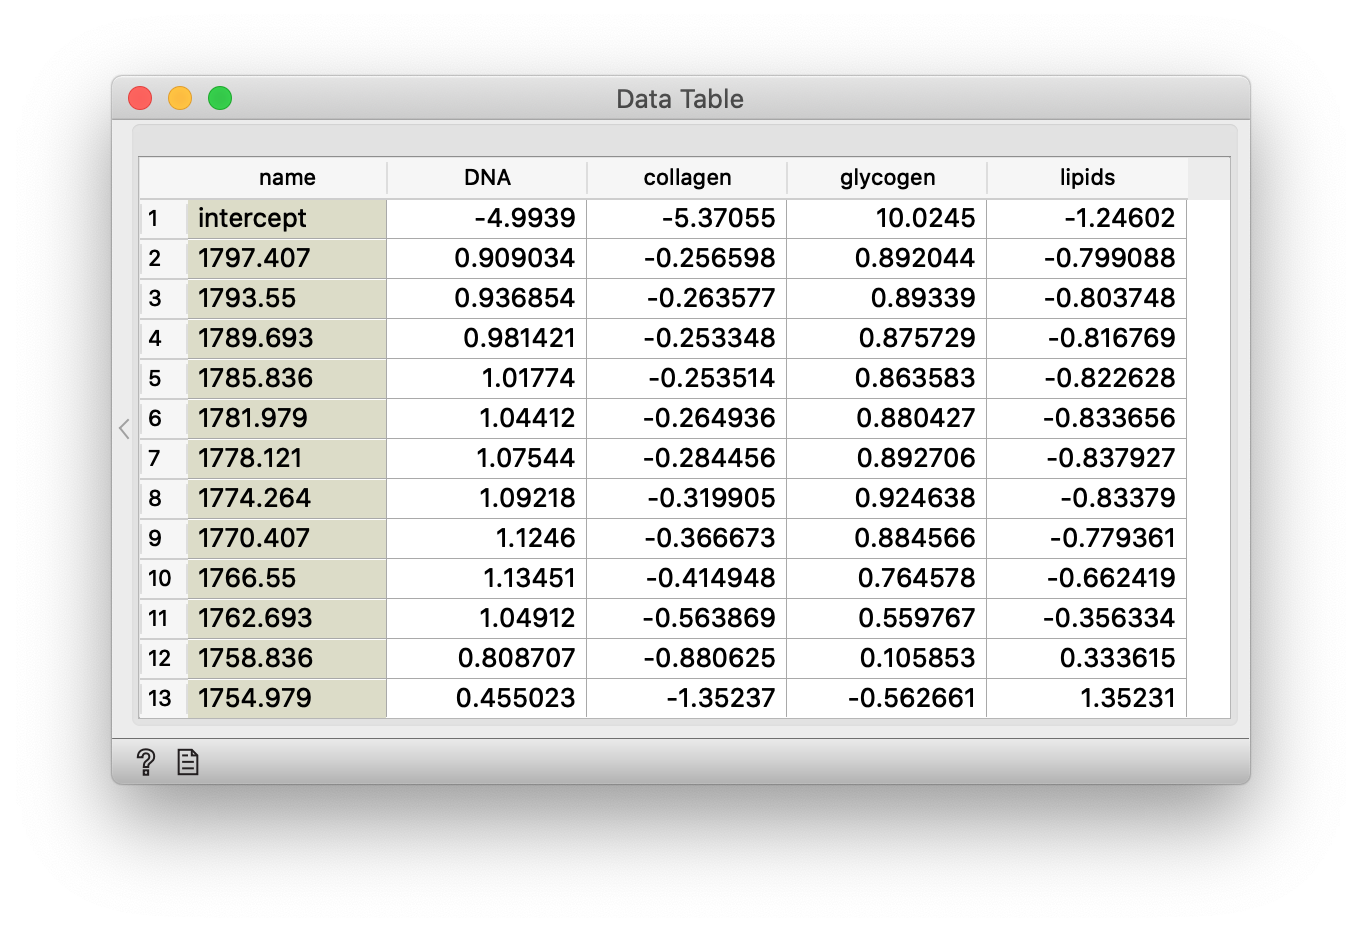
\includegraphics[width=0.9\textwidth]{graphics/ch-spectra_classification/sp_classification-fig4.png}
  \label{fig:spectra_classification-fig4}
\end{wrapfigure}
We get a table that is hard to understand. What if we visualize it? First, \widget{Transpose} the data. Then, use \widget{Select Columns} to make the visualization prettier: in the widget remove the intercept.

Now, open \widget{Logistic Regression} and try changing its parameters. Observe the effect on the weights.

\begin{figure}[h]
\hspace{-1cm}\stackinset{r}{0\linewidth}{t}{-0.22\linewidth}
  {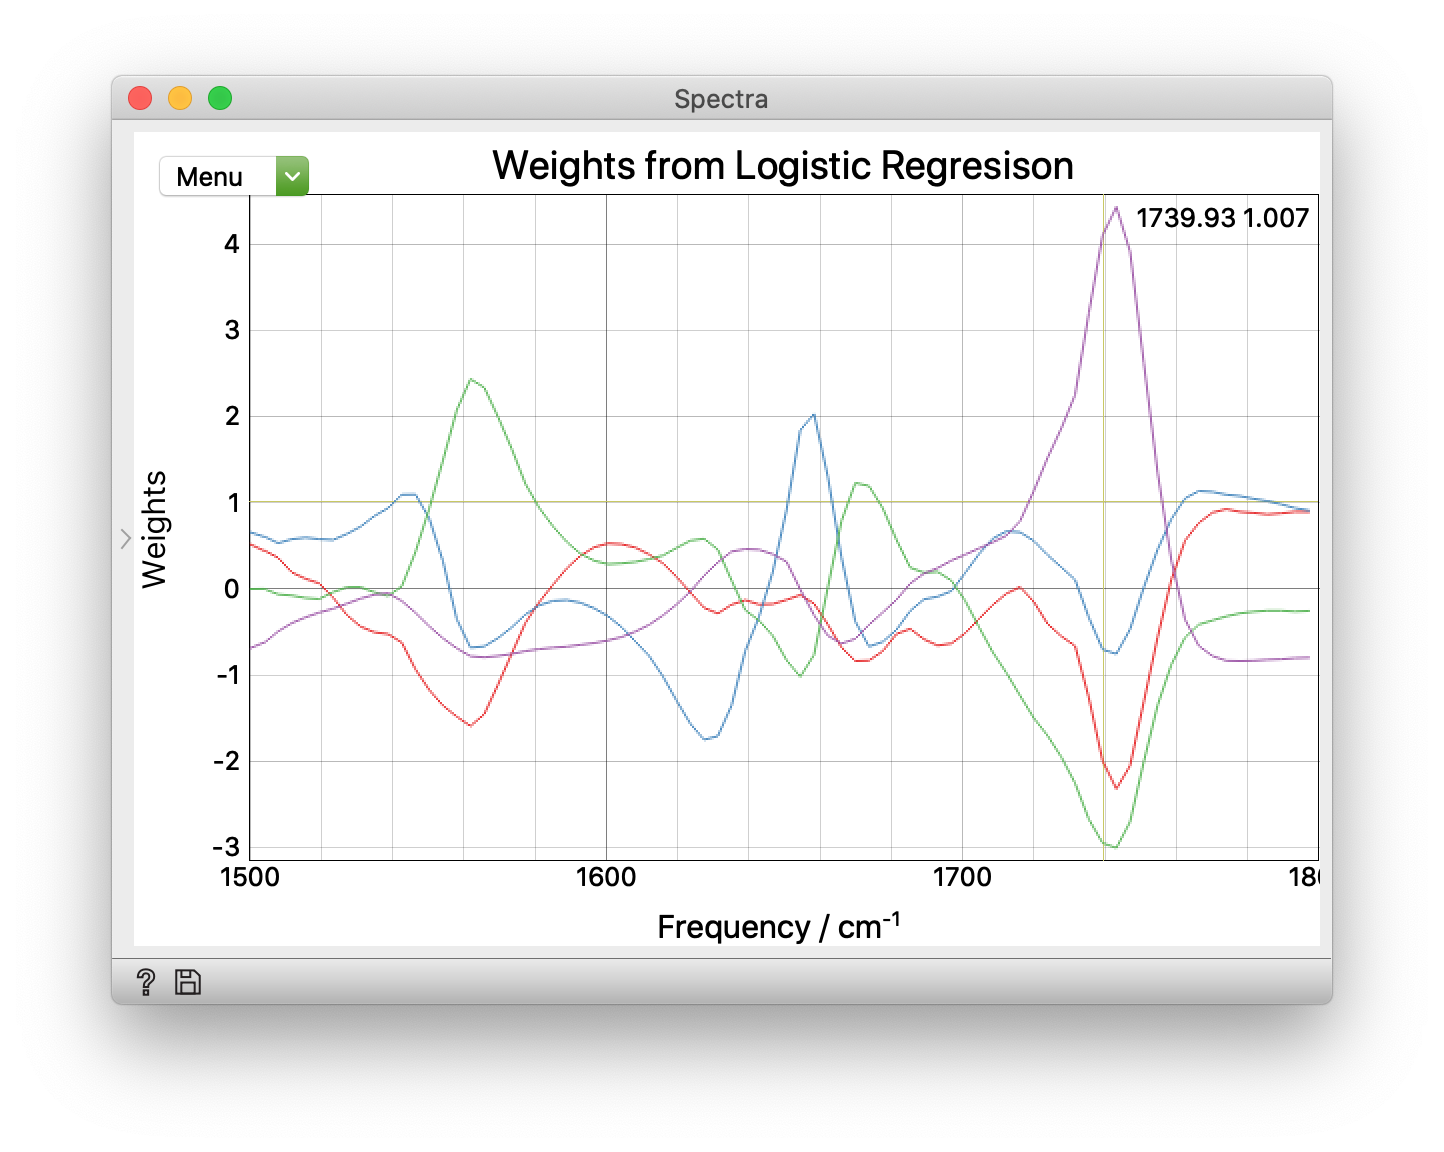
\includegraphics[scale=0.35]{graphics/ch-spectra_classification/sp_classification-fig5a.png}}
  {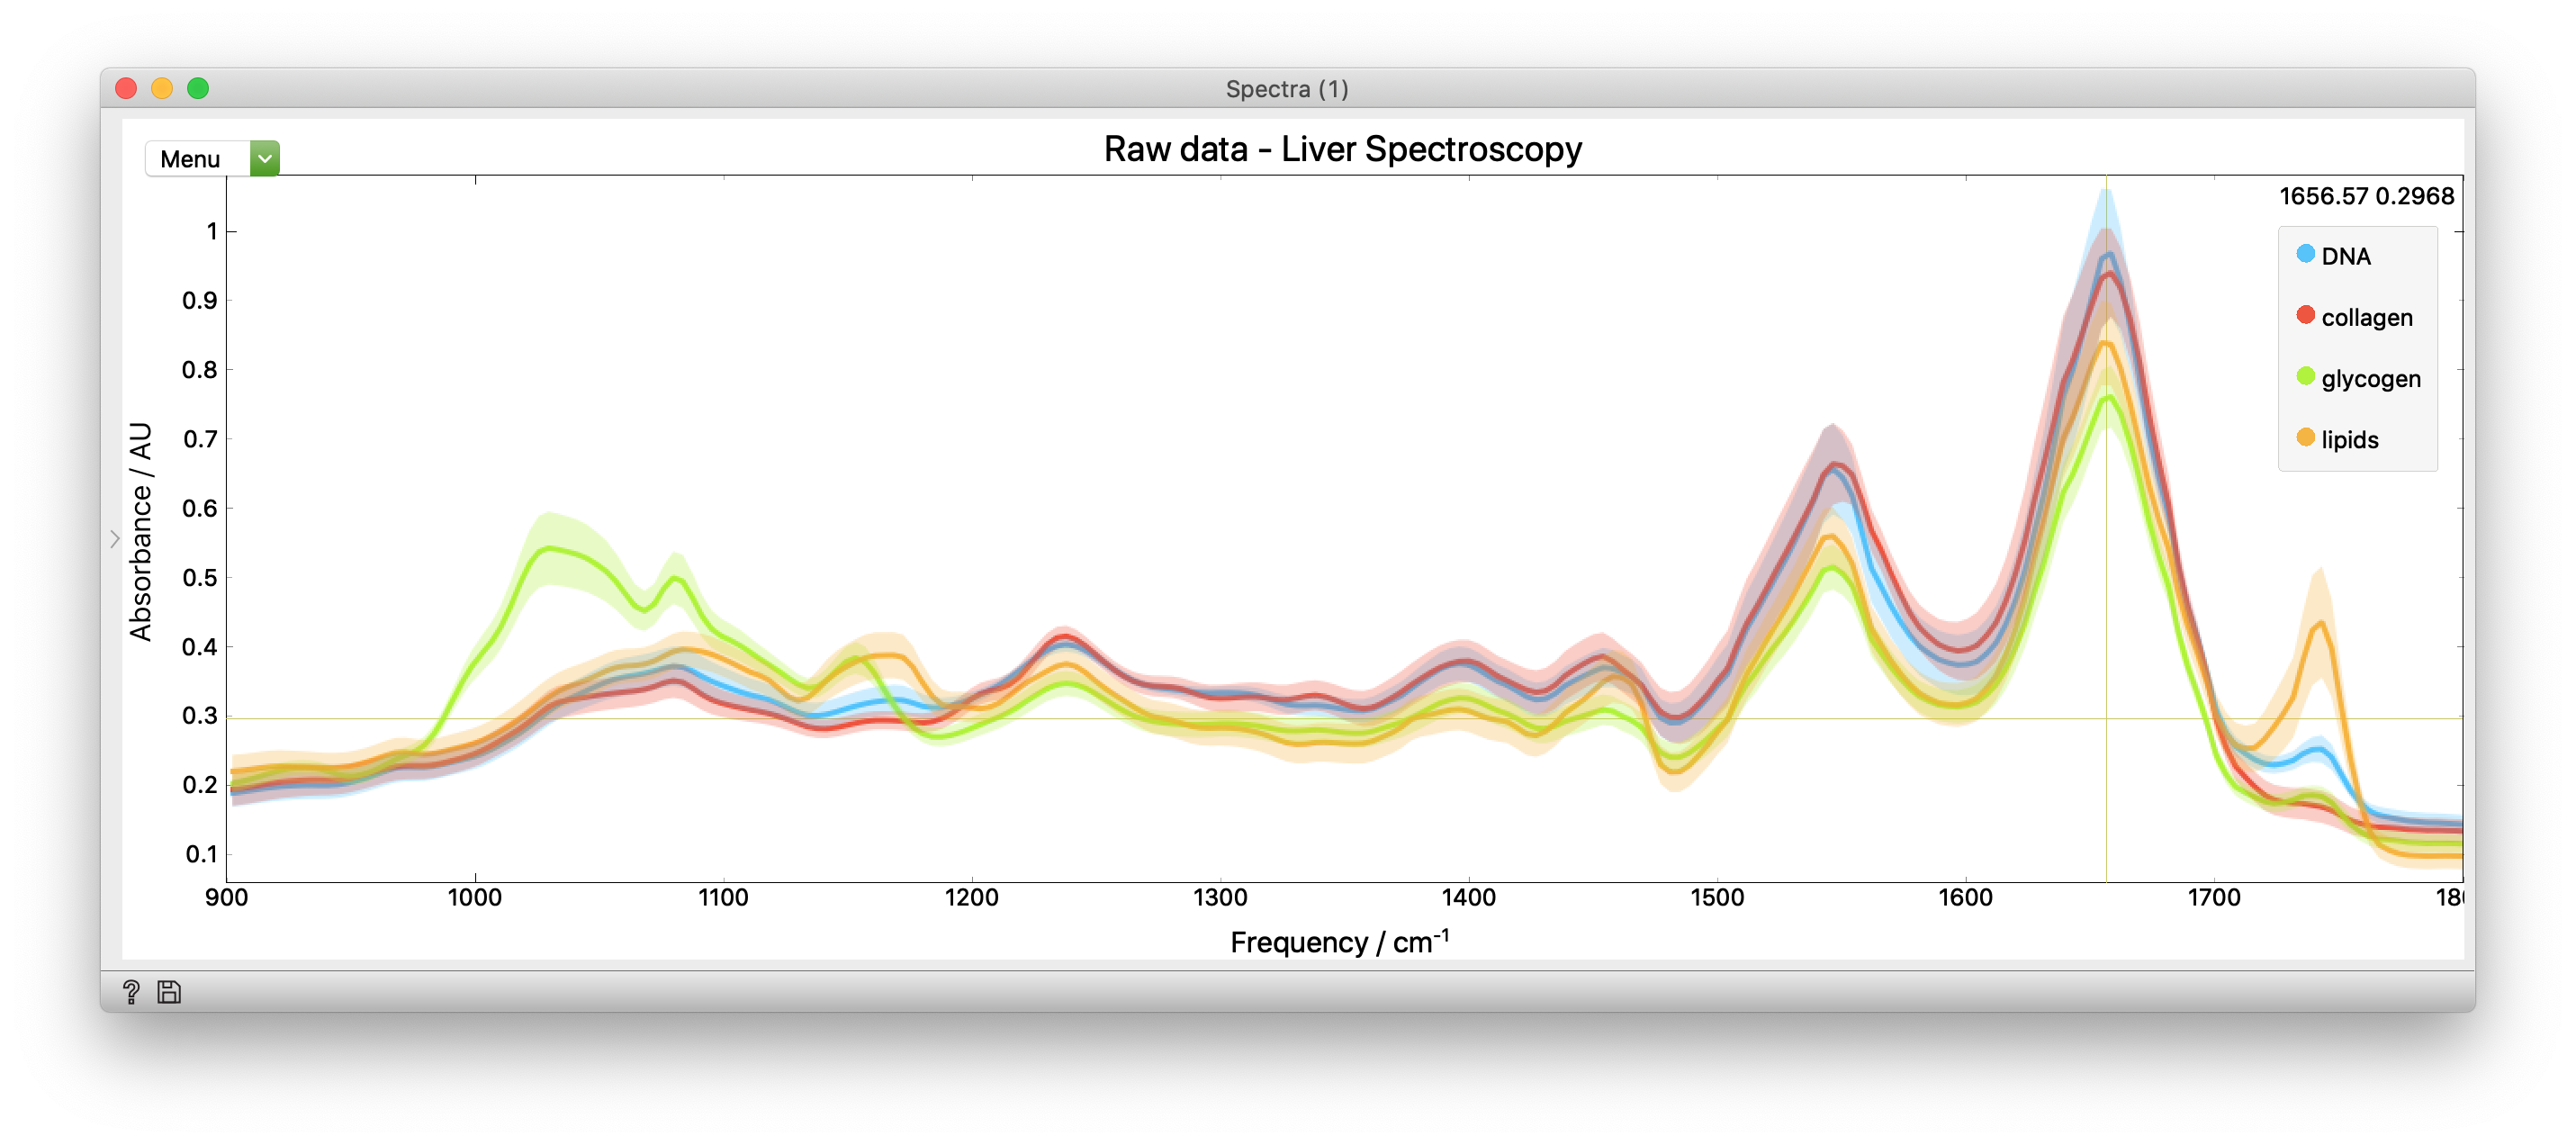
\includegraphics[scale=0.35]{graphics/ch-spectra_classification/sp_classification-fig5b.png}}
  \label{fig:spectra_classification-fig5}
\end{figure}

%TODO Marko % Lesson 21: New and Different Test Data
% Lesson 22: Clustering Spectral Images
\chapter{Clustering Spectral Images}
\label{ch:spectra_image_clustering}

\begin{wrapfigure}{o}{0.63\textwidth}
    \centering
    \vspace{-3.3cm}
    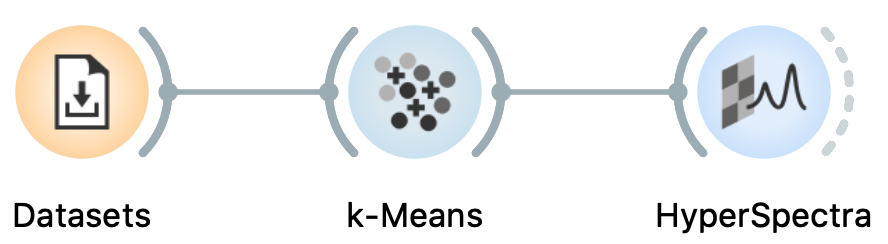
\includegraphics[width=0.75\textwidth]{graphics/ch-spectra_image_clustering/sp_image_clustering-fig1.png}
    \label{fig:spectra_image_clustering-fig1}
\end{wrapfigure}

We have already seen hierarchical clustering. Another clustering algorithm, k-Means, is much faster for data with lots of rows, like images, which contain a row (a spectrum) for each pixel. Still, for the liver-cirrhosis data, both approaches are fast. Here, we use \widget{k-Means} with k=3 clusters. 

\begin{figure}[h]
\vspace{-0.5cm}
\hspace{-1cm}\stackinset{r}{-1.15\linewidth}{t}{0.025\linewidth}
  {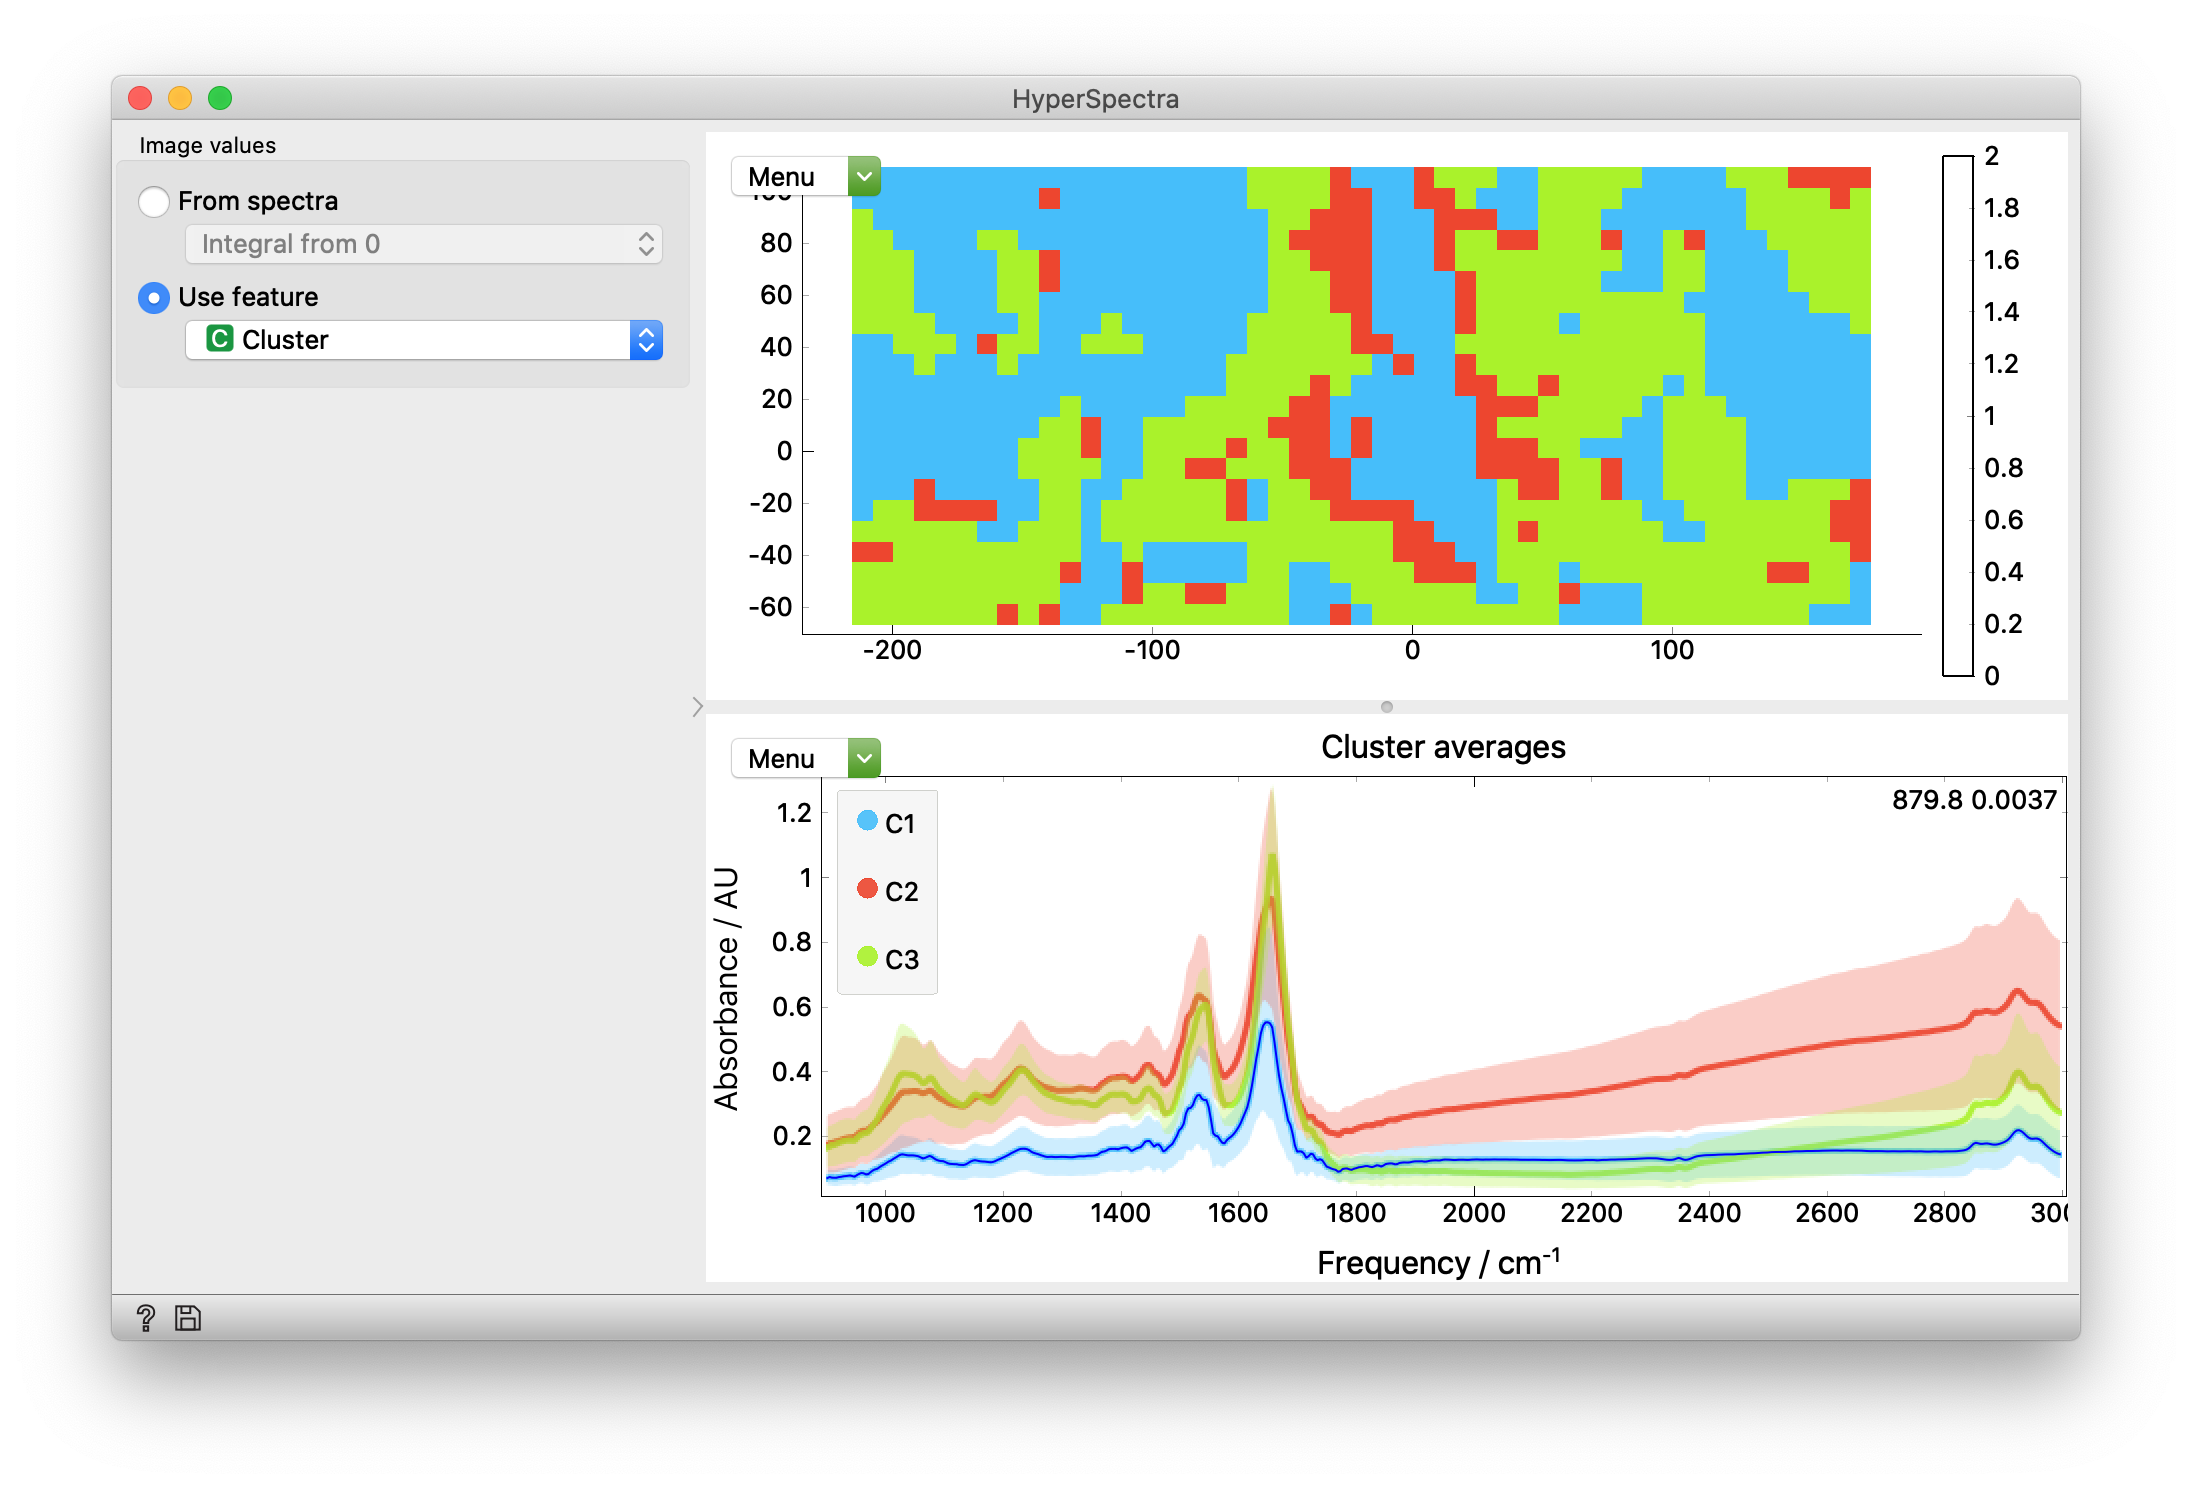
\includegraphics[scale=0.33]{graphics/ch-spectra_image_clustering/sp_image_clustering-fig2b.png}}
  {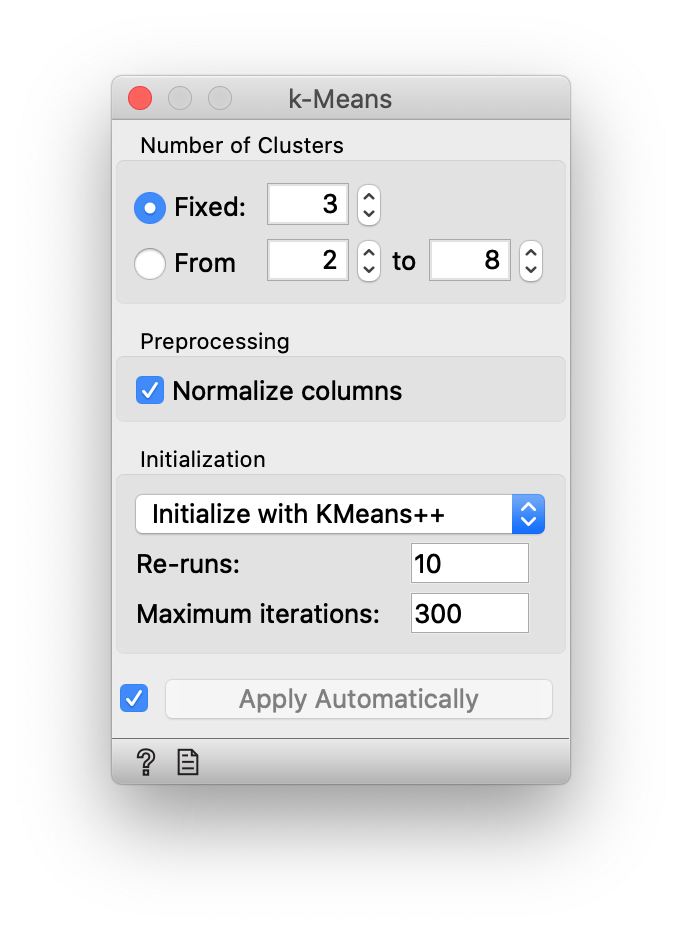
\includegraphics[scale=0.55]{graphics/ch-spectra_image_clustering/sp_image_clustering-fig2a.png}}
%  \caption{The \widget{Spectra} widget shows wrong predictions for the DNA class.}
  \label{ffig:spectra_image_clustering-fig2}
\end{figure}



\begin{wrapfigure}{o}{1.1\textwidth}
  \centering
  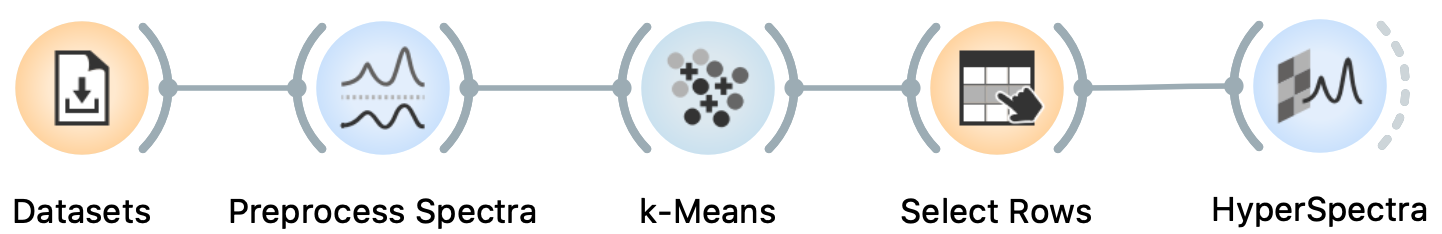
\includegraphics[width=1.1\textwidth]{graphics/ch-spectra_image_clustering/sp_image_clustering-fig3.png}%
  \label{fig:spectra_image_clustering-fig3}
\end{wrapfigure}
We see no meaningful clusters. Therefore, we need to preprocess the data. If we do it well, we see that a cluster corresponds to the background. We could remove it with the Select Rows widget.

\begin{wrapfigure}{o}{0.9\textwidth}
%  \centering
  \vspace{-0.5cm}
  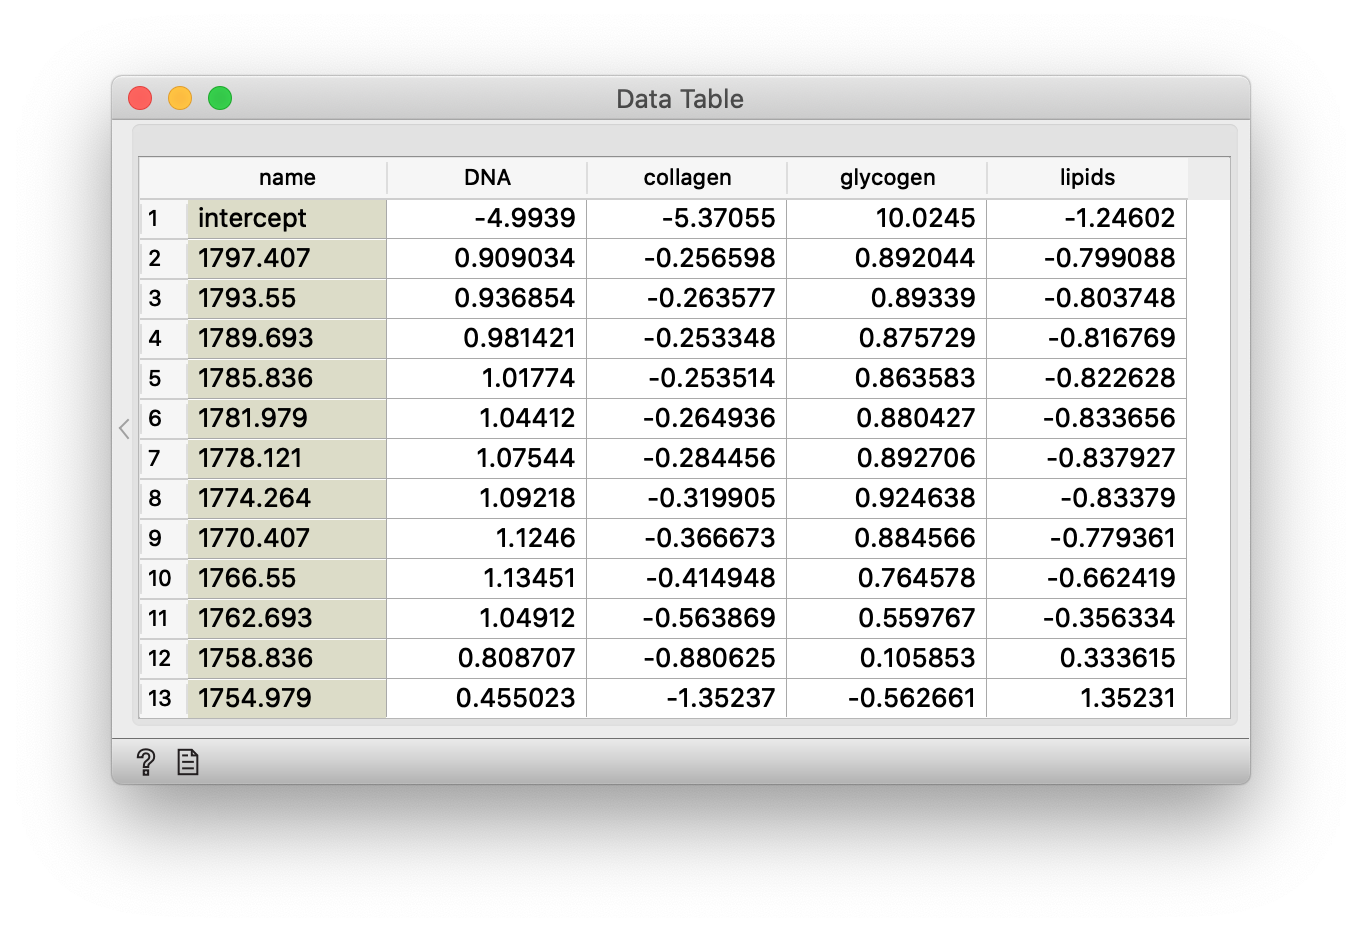
\includegraphics[width=0.9\textwidth]{graphics/ch-spectra_classification/sp_classification-fig4.png}
  \label{fig:spectra_classification-fig4}
\end{wrapfigure}

%TODO Feri % Lesson 23: PCA with Spectral Images
%TODO Feri % Lesson 24: Classification on Hyperspectral Images
%TODO Feri % Lesson 25: Preprocessing with EMSC
%TODO Feri % Lesson 26: Adding Annotations
% Lesson 27: Visualizing similarities based on various metrics (Neighbors widget)
\chapter{Visualize spectral distances}
\label{ch:visualize-spectral-distances}

\begin{wrapfigure}{o}{0.65\textwidth}
	\vspace{-1.5 cm}
    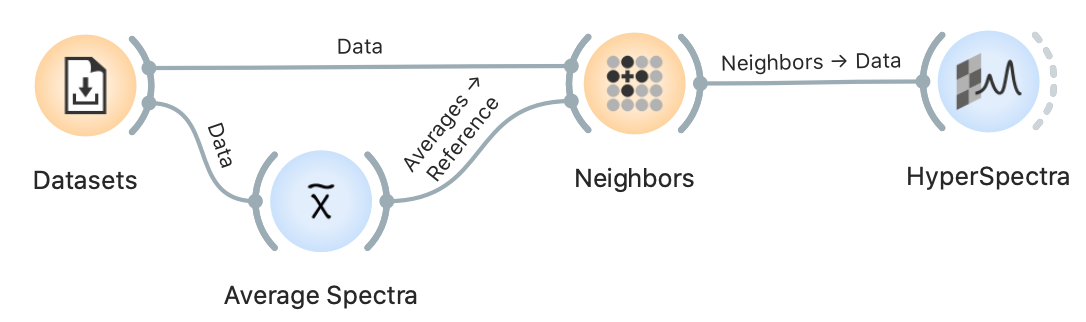
\includegraphics[scale=0.6]{graphics/ch-visualize_spectral_distances/ch-visualize_spectral_distances-fig1.png}
\end{wrapfigure}

Let's consider a spectrum, or any other data entry for that matter, as a point in a multidimensional space. We can define distance metrics between these points and visualize the distance values from one another or from a selected reference point or reference spectrum. By doing so, we can explore how similar our measurements are to a selected reference. We can do this on a series of spectra or even on hyperspectral maps!

If you build the workflow shown above this paragraph in \mutation\ you will be able to explore various distance metrics. First, let's use the \textit{'Liver cirrhosis - spectral image'} dataset provided by the \widget{Datasets} widget, then calculate the \textit{Euclidean distances} from the average spectrum with the \widget{Neighbors} widget and visualize them in \widget{Hyperspectra}. 

\medskip
Can you reproduce the results below? Pay attention to the color scheme.

\begin{figure*}[h]
\centering
\infinitewidthbox{
  \stackinset{r}{-0.5\linewidth}{t}{+0.1\linewidth}
  {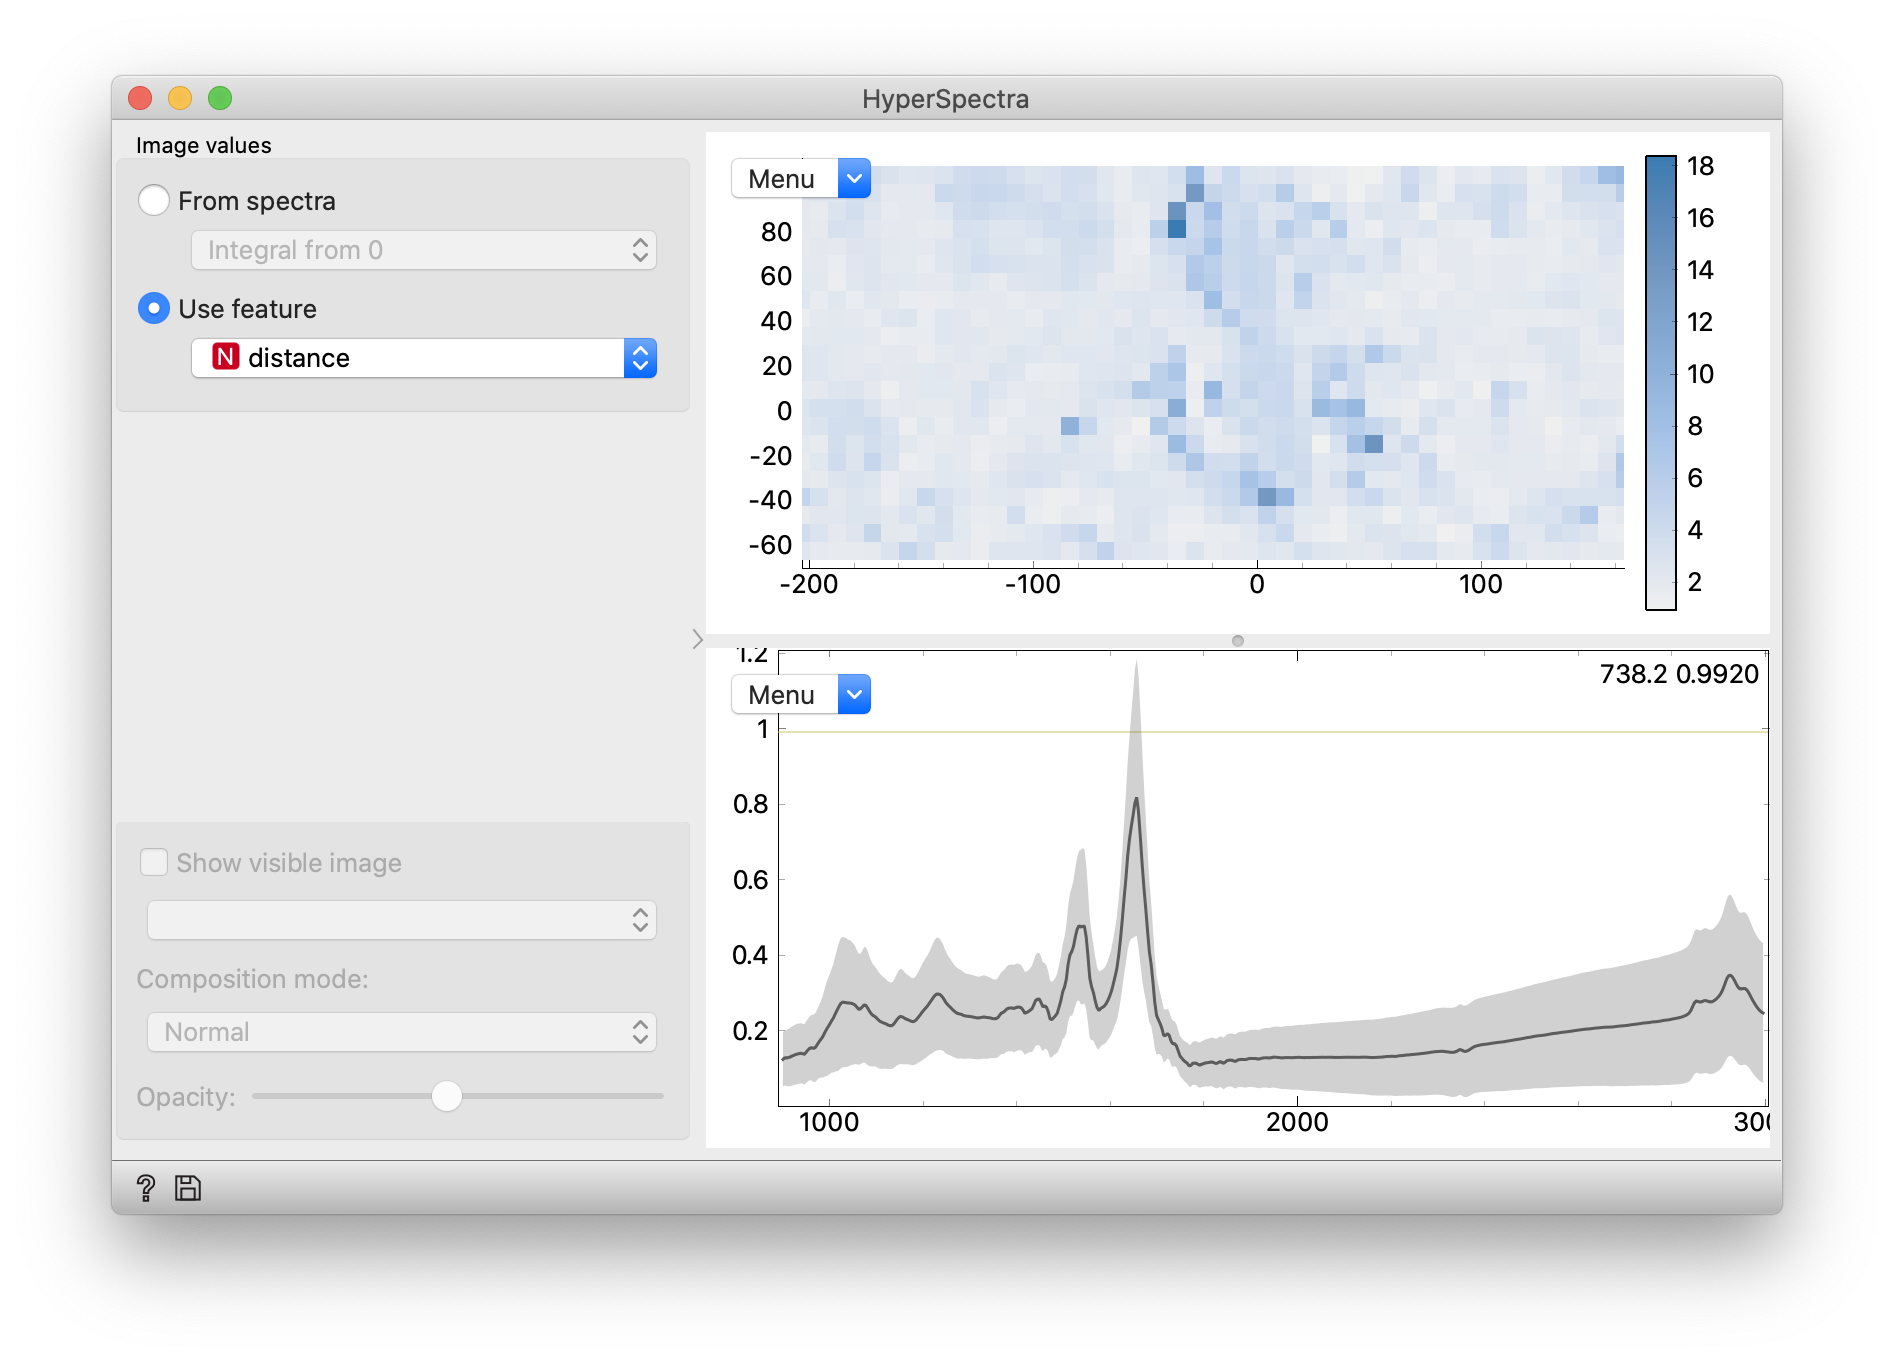
\includegraphics[scale=0.4]{graphics/ch-visualize_spectral_distances/ch-visualize_spectral_distances-fig3.png}}
  {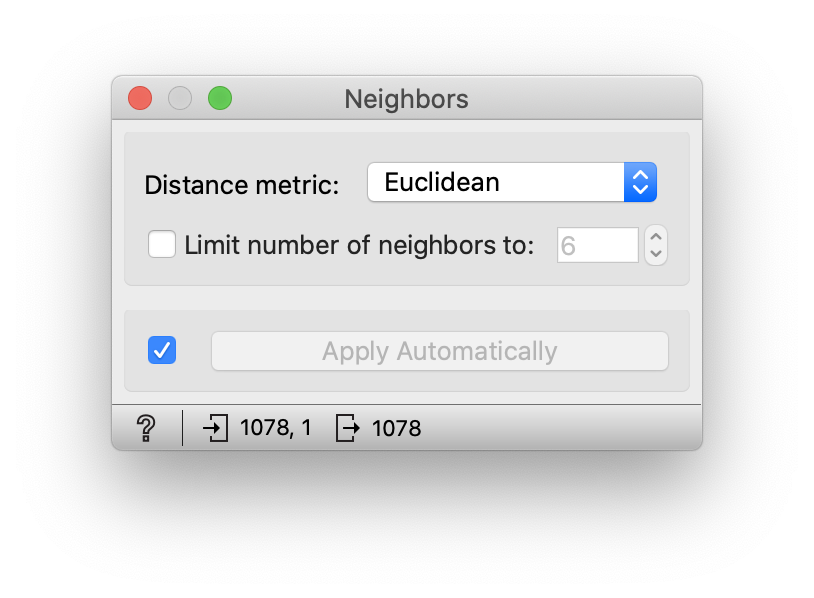
\includegraphics[scale=0.6]{graphics/ch-visualize_spectral_distances/ch-visualize_spectral_distances-fig2.png}}
  \hspace{8cm}
  }
%\caption{Try changing the parameters!}

\end{figure*}

Explore different distance metrics, inspect distances in a \widget{Data Table} widget. Don't forget, you can select points on the top map and see the corresponding spectra on the bottom in \widget{Hyperspectra}. 

% I would like to have a special environment called notes for example that we can switch on or off to print or hide lecturer notes.
\lecnotes{Possibility for discussion of the general mathematical properties of distance functions. See \url{https://en.wikipedia.org/wiki/Metric_(mathematics)}}
%%
% The back matter contains appendices, bibliographies, indices, glossaries, etc.
\backmatter

\bibliography{sample-handout}
\bibliographystyle{plainnat}


\printindex

\end{document}
